%
% $Id: $
%
%
% Compilar a .pdf con LaTeX (pdflatex)
% Es necesario instalar Beamer (paquete latex-beamer en Debian)
%

%
% Gr�ficos:
% Los gr�ficos pueden suministrarse en PNG, JPG, TIF, PDF, MPS
% Los EPS deben convertirse a PDF (usar epstopdf)
%

\documentclass{beamer}
\usetheme{Warsaw}
%\usebackgroundtemplate{
\includegraphics[width=\paperwidth]{format/libresoft-bg.png}}
%\usepackage[spanish]{babel}
\usepackage[latin1]{inputenc}
\usepackage{graphics}
\usepackage{amssymb} % Simbolos matematicos
\usepackage{url}
\usepackage{multirow}


%\definecolor{libresoftgreen}{RGB}{162,190,43}
%\definecolor{libresoftblue}{RGB}{0,98,143}

%\setbeamercolor{titlelike}{bg=libresoftgreen}

%% Metadatos del PDF.
\hypersetup{
  pdftitle={How social are Scratch learners? A comprehensive analysis of the Scratch platform for social interactions},
  pdfauthor={J. Moreno-Le�n, Gregorio Robles, Marcos Rom�n-Gonz�lez},
  pdfcreator={GSyC/LibreSoft \\ Universidad Rey Juan Carlos},
  pdfproducer=PDFLaTeX,
  pdfsubject={Code to learn with Scratch},
}
%%

\begin{document}

\title{How social are Scratch learners?}
\subtitle{A comprehensive analysis of the Scratch platform for social interactions}
\institute{jesus.moreno@programamos.es, grex@gsyc.urjc.es, mroman@edu.uned.es \\
GSyC/Libresoft, Universidad Rey Juan Carlos}
\author{J. Moreno-Le�n, Gregorio Robles, Marcos Rom�n-Gonz�lez}
\date{FLOSSEdu workshop @ OSS 2016, Gothenburg, June 2\textsuperscript{nd} 2016}

\frame{
\maketitle
\begin{center}

\includegraphics[width=2cm]{format/libresoft-logo}
\hspace{0.5cm}

\includegraphics[width=5cm]{format/gsyc-urjc}
\vspace{0.5cm}

\includegraphics[width=3cm]{format/emadrid.png}
\end{center}
}


% Si el titulo o el autor se quieren acortar para los pies de p�gina
% se pueden redefinir aqu�:
%\title{Titulo corto}
%\author{Autores abreviado}

%% LICENCIA DE REDISTRIBUCION DE LAS TRANSPAS
\frame{
~
\vspace{3cm}

\begin{flushright}

\includegraphics[width=2.2cm]{figs/by-sa}

{\tiny
(cc) 2016 J. Moreno-Le�n, Gregorio Robles and Marcos Rom�n-Gonz�lez\\
  Some rights reserved. This work licensed under Creative Commons \\
  Attribution-ShareAlike License. To view a copy of full license, see \\
  http://creativecommons.org/licenses/by-sa/3.0/ or write to \\
  Creative Commons, 559 Nathan Abbott Way, Stanford, \\
  California 94305, USA. \\
\ \\
Some of the figures have been taken from the Internet \\
Source, and author and licence if known, is specified. \\
For those images, \emph{fair use} applies.
}
\end{flushright}
}
%%

\section{FLOSSEdu workshop, Gothenburg}


%--------------------------------------------------------
%\usebackgroundtemplate{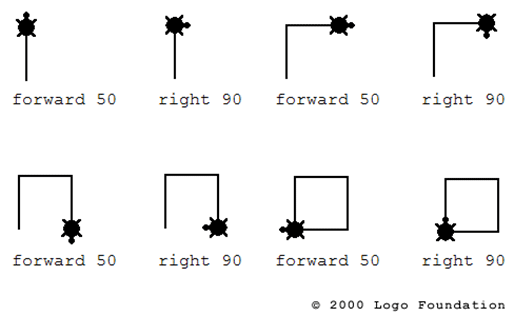
\includegraphics[height=10cm]{figs/turtles.png}}
% background: http://www.wim-network.org/wp-content/uploads/2012/04/iceberg.jpg

\begin{frame}
\frametitle{}
\end{frame}

\usebackgroundtemplate{}
%--------------------------------------------------------
%\usebackgroundtemplate{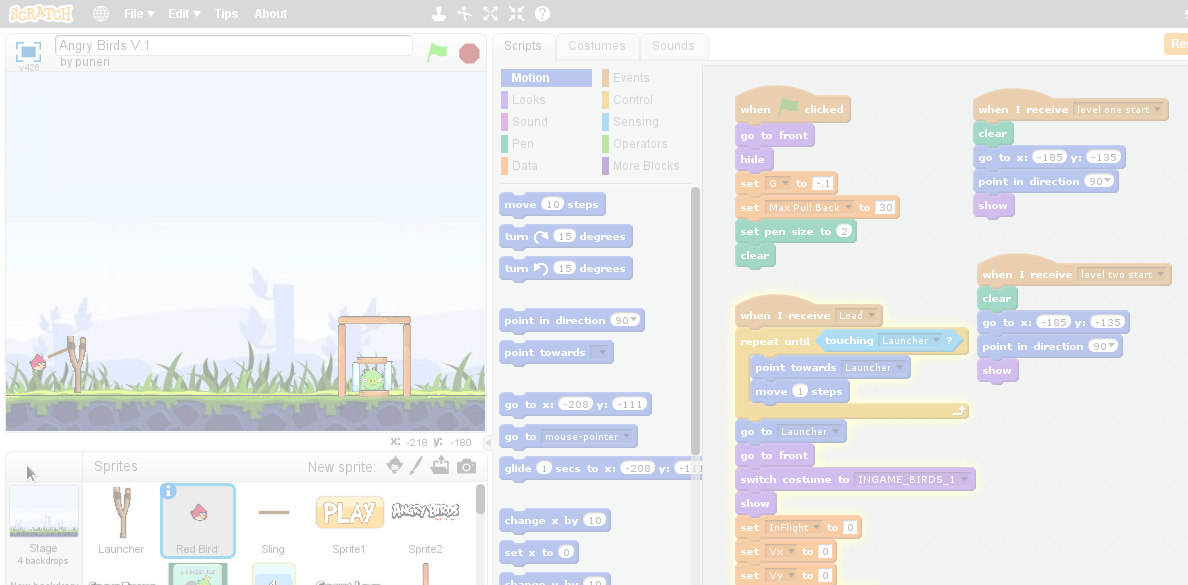
\includegraphics[width=18cm]{figs/AngryBirds2.png}}
\begin{frame}
\frametitle{}

\end{frame}
\usebackgroundtemplate{}
%--------------------------------------------------------
\frame{
\maketitle
\begin{center}

\includegraphics[width=2cm]{format/libresoft-logo}
\hspace{0.5cm}

\includegraphics[width=5cm]{format/gsyc-urjc}
\vspace{0.5cm}

\includegraphics[width=3cm]{format/emadrid.png}
\end{center}
}

\end{document}
